\documentclass{article}

\usepackage{graphicx}
\usepackage{tikz}
\usepackage{tikzsymbols}
\usetikzlibrary{calc,patterns,shapes.geometric}
\pagestyle{empty}
\usepackage[margin=0pt]{geometry}
\geometry{papersize={14in,12in}}

\def\centerarc[#1](#2)(#3:#4:#5){\draw[#1] ($(#2)+({#5*cos(#3)},{#5*sin(#3)})$) arc (#3:#4:#5);}

\begin{document}
	\begin{figure}
		\centering
		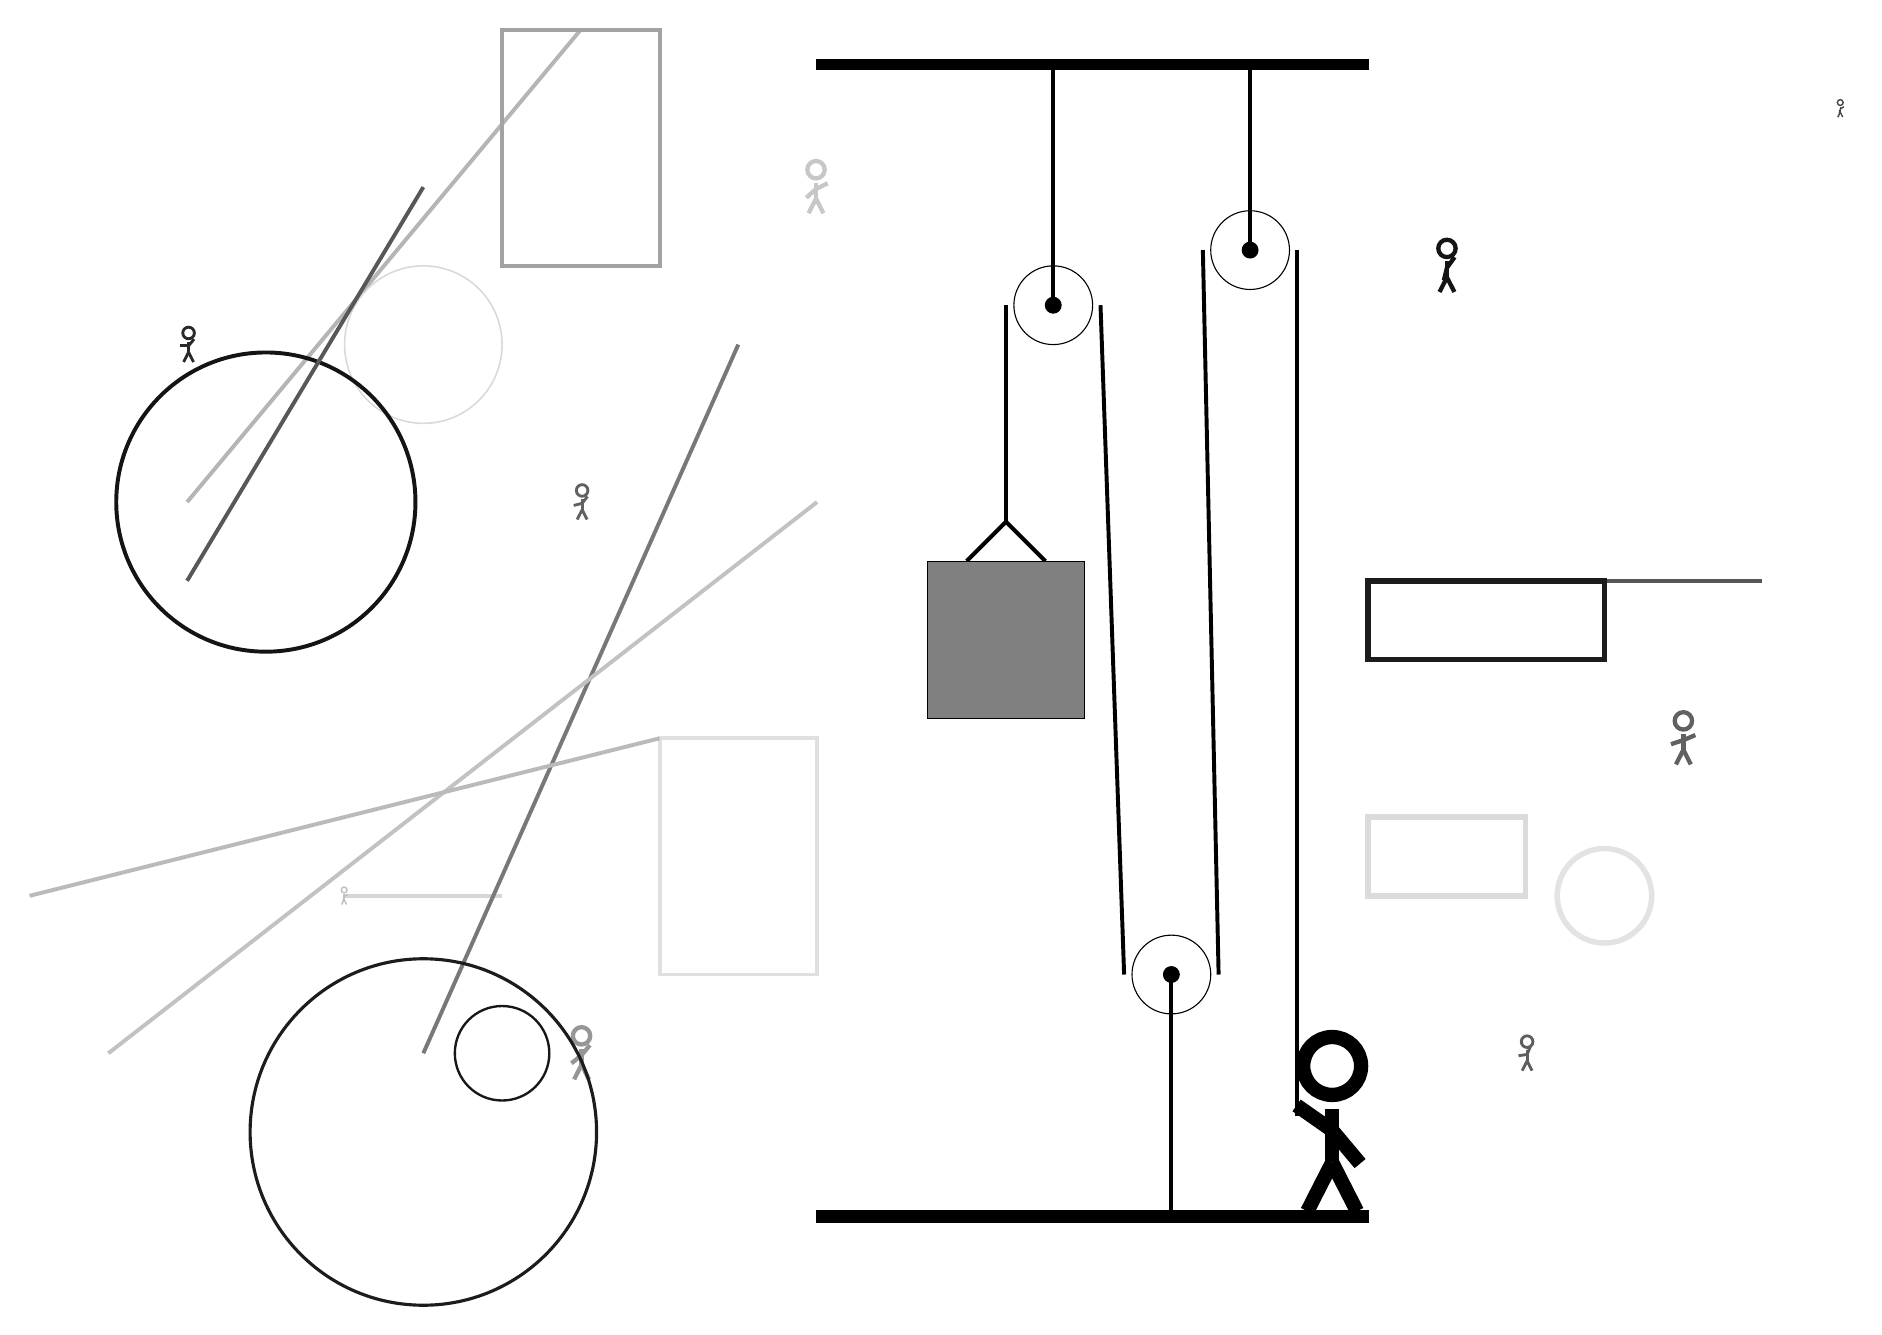
\begin{tikzpicture}
			%%%%% START %%%%%
			
			\draw[fill=black] (-2, 11.5) rectangle (5, 11.625);
			
			\draw (1, 8.5) circle (0.5);
			\draw[fill=black] (1, 8.5) circle (0.1);
			\draw[line width=0.5mm]  (1, 11.5) -- (1, 8.5);
			
			\draw[fill=white](2.5, 0.0) circle (0.5);
			\draw[fill=black] (2.5, 0.0) circle (0.1);
			\draw[line width=0.5mm]  (2.5, -3) -- (2.5, 0.0);
			
			\draw[fill=white](3.5, 9.2) circle (0.5);
			\draw[fill=black] (3.5, 9.2) circle (0.1);
			\draw[line width=0.5mm] (3.5, 11.5) -- (3.5, 9.2);
			
			\draw[line width=0.5mm, color=black!29](-5, 12) -- (-10, 6);
			
			\node[line width=0.7mm, color=black!72] at (11, 11) {\Strichmaxerl[1][77][32]};
			\draw [line width=0.2mm, color=black!15](-7, 8) circle (1.0);
			\draw[line width=0.5mm, color=black!36] (-4, 12) rectangle (-6, 9);
			\draw [line width=0.5mm, color=black!92](-9, 6) circle (1.9);
			\draw[line width=0.5mm, color=black!12] (-2, 3) rectangle (-4, 0);
			\draw[line width=0.5mm, color=black!66](7, 5) -- (10, 5);
			\draw[line width=0.5mm, color=black!16](-6, 1) -- (-8, 1);
			\draw [line width=0.3mm, color=black!91](-6, -1) circle (0.6);
			\draw [line width=0.7mm, color=black!11](8, 1) circle (0.6);
			\node[line width=0.6mm, color=black!41] at (-5, -1) {\Strichmaxerl[3][39][50]};
			\draw[line width=0.5mm, color=black!53](-3, 8) -- (-7, -1);
			\node[line width=0.7mm, color=black!62] at (-5, 6) {\Strichmaxerl[2][14][52]};
			
			\draw[line width=0.5mm, color=black!24](-2, 6) -- (-11, -1);
			\node[line width=0.4mm, color=black!84] at (-10, 8) {\Strichmaxerl[2][0][51]};
			\draw[line width=0.7mm, color=black!14] (5, 2) rectangle (7, 1);
			\node[line width=0.6mm, color=black!92] at (6, 9) {\Strichmaxerl[3][76][54]};
			\node[line width=0.7mm, color=black!22] at (-2, 10) {\Strichmaxerl[3][42][26]};
			\node[line width=0.7mm, color=black!62] at (9, 3) {\Strichmaxerl[3][18][23]};
			\draw[line width=0.7mm, color=black!89] (5, 4) rectangle (8, 5);
			\draw [line width=0.4mm, color=black!89](-7, -2) circle (2.2);
			
			\draw[line width=0.5mm, color=black!27](-4, 3) -- (-12, 1);
			\node[line width=0.7mm, color=black!63] at (7, -1) {\Strichmaxerl[2][8][68]};
			\draw[line width=0.5mm, color=black!66](-7, 10) -- (-10, 5);
			\node[line width=0.5mm, color=black!25] at (-8, 1) {\Strichmaxerl[1][76][26]};
			
			
			\draw[line width=0.5mm] (-0.1, 5.25) -- (0.4, 5.75) -- (0.9, 5.25);
			\draw[fill=black!50] (-0.6, 5.25) rectangle (1.4, 3.25);
			
			\draw[line width=0.5mm] (0.4, 8.5) -- (0.4, 5.75);
			\centerarc[line width=0.5mm](1, 8.5)(0:180:0.6);
			\draw[line width=0.5mm](1.6, 8.5) -- (1.9, 0.0);
			\centerarc[line width=0.5mm](2.5, 0.0)(180:360:0.6);
			\draw[line width=0.5mm](3.1, 0.0) -- (2.9, 9.2);
			\centerarc[line width=0.5mm](3.5, 9.2)(0:180:0.6);
			\draw[line width=0.5mm](4.1, 9.2) -- (4.1, -1.8);
			
			\node at (4.5, -1.9) {\Strichmaxerl[10][-35][-50]};
			
			\draw[fill=black] (-2, -3) rectangle (5, -3.15);
			
			%%%%% END %%%%%
		\end{tikzpicture}
	\end{figure}	
\end{document}